\begin{center}[15.]\par\medskip\textit{Kugelfläche.}\end{center}
Seien $x,y,z$ die Koordinaten eines Punkts auf einer Linie, die auf der Kugelfläche liegt und in sich selbst zurückkehrt. $xx+yy+zz=rr$

Das Integral
\[
\int\frac{z(x\mathrm dy-y\mathrm dx)}{r(xx+yy)}=V
\]
ist über die ganze Länge der Linie zu nehmen.

Diese Linie teilt die Kugelfläche in zwei oder mehr Teile $A,B,C$ usw.

Dann gilt
\[
V=\alpha A+\beta B+\gamma C+\,.\,.
\]
wobei die Koeffizienten $\alpha,\beta,\gamma,\,.\,.$ die folgenden beiden Bedingungen erfüllen.

1.\quad Die Koeffizienten zweier benachbarter Teile unterscheiden sich stets um eine Einheit. Der kleinere Koeffizient gehört zu dem Teil, der zur Trennlinie so liegt wie der positive Pol der $z$ zum Großkreis, der vom Pol der $x$ zum Pol der $y$ gezogen ist.

2.\quad Die Summe der Koeffizienten derjenigen Teile, in denen die beiden Pole der $z$ liegen, ist $=0$.

Das lässt sich leicht beweisen, indem man vom negativen zum positiven Pol der $z$ unendlich viele Halbkreise zieht.

Der Fall, dass einer der beiden Pole auf der Linie selbst liegt, ist durch die Natur des Integrals von selbst ausgeschlossen.

\SourceLeaf{627}
\begin{center}[16.]\par\medskip\textit{Elektromotorische Kraft durch die Entstehung eines Stroms.}\end{center}
\begin{center}\begin{tikzpicture}[x=.105mm,y=.105mm,line width=.65pt]
  \coordinate (origin) at (0,0);
  \coordinate (P) at (0,114);
  \coordinate (A) at (239,0);
  \coordinate (B) at (1027,0);
  \draw[dash pattern=on 2.5pt off 2pt] (P)--(origin)--(A);
  \draw (A)--(B);
  \fill (P) circle[radius=2pt];
  \node[above=3pt,inner sep=0pt] at (P) {\bfseries P};
  \node[below=3pt,inner sep=0pt] at (origin) {\bfseries O};
  \node[below=3pt,inner sep=0pt] at (A) {\bfseries A};
  \node[right=4pt,inner sep=0pt] at (B) {\bfseries B};
\end{tikzpicture}
\end{center}
Elektromotorische Kraft in $P$ infolge der Entstehung des Stroms in $A\, .\, .\, .\, B$
\[
=\log\frac{x'+\BareRoot{(x'x'+yy)}}{x^0+\BareRoot{(x^0x^0+yy)}},\quad\text{wenn}\quad0A=x^0,\quad0B=x',\quad0P=y
\]

Elektromotorische Kraft in $P$ infolge der Entstehung eines Stroms durch den Kreis
\begin{center}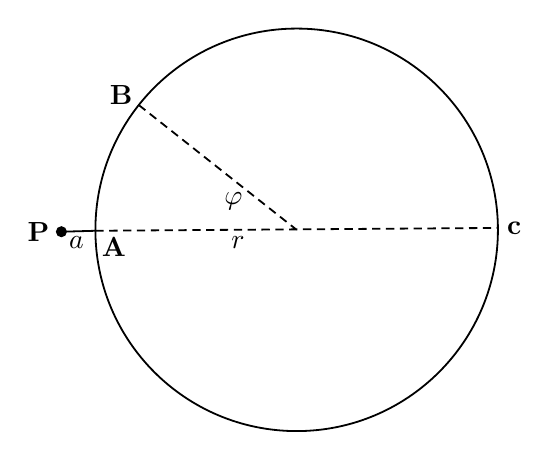
\begin{tikzpicture}[x=.12mm,y=.12mm,line width=.65pt]
  \coordinate (center) at (0,0);
  \coordinate (P) at (-249,-2);
  \coordinate (A) at (-213,-1);
  \coordinate (B) at (-167,132);
  \coordinate (c) at (213,2);
  \draw (center) circle[radius=25.56mm];
  \draw (P)--(A);
  \draw[dash pattern=on 3pt off 2pt] (A)--(c) (B)--(center);
  \fill (P) circle[radius=2pt];
  \node[left=4pt,inner sep=0pt] at (P) {\bfseries P};
  \node[anchor=north west,xshift=2pt,yshift=-2pt,inner sep=0pt] at (A) {\bfseries A};
  \node[anchor=south east,xshift=-2pt,inner sep=0pt] at (B) {\bfseries B};
  \node[right=3pt,inner sep=0pt] at (c) {\bfseries c};
  \node[below=2pt,inner sep=0pt] at (-233,0) {$a$};
  \node[below=2pt,inner sep=0pt] at (-62,0) {$r$};
  \node[above=1pt,inner sep=0pt] at (-67,17) {$\varphi$};
\end{tikzpicture}
\end{center}
\[
\begin{aligned}
&\text{1) durch das Stück }AB\,.\,.\text{ näherungsweise }\log\frac{2r\sin\varphi}{a}\\
&\text{2) durch das Stück }BC\text{ näherungsweise }-2-\log\operatorname{tg}\tfrac14\varphi\\
&\text{Zusammen}\quad\log\frac{8r\varphi}{a}-2=\log\frac{8r\varphi}{aee}\\
&\text{Durch den ganzen Kreis}\quad2\log\frac{8r}{aee}
\end{aligned}
\]

\begin{center}[17.]\end{center}
Durch die Drehung eines Kreises mit dem Radius $=\rho$ um eine in seiner Ebene liegende Achse entstehe ein ringförmiger Körperraum. Der Mittelpunkt des Kreises habe von der Achse den Abstand $=R$, und der Raum sei gleichmäßig mit einer Rheophorkette ausgefüllt. Die Anzahl der Windungen sei $M$. Es wird angenommen, dass $\rho$ im Verhältnis zu $R$ sehr klein ist. Gesucht ist die elektromotorische Wirkung des Rings auf einen Punkt, der entweder innerhalb des Rings oder sehr nahe an ihm liegt.
\begin{center}\begin{tikzpicture}[x=.12mm,y=.12mm,line width=.65pt]
  \coordinate (center) at (0,0);
  \coordinate (axisMid) at (525,0);
  \coordinate (axisTop) at (525,190);
  \coordinate (axisBottom) at (525,-167);
  \draw (center) circle[radius=16.32mm];
  \draw[dash pattern=on 3pt off 2pt] (center)--(axisMid) (axisTop)--(axisBottom);
\end{tikzpicture}
\end{center}

Sei $a$ der Abstand des Punkts von der Mittellinie des Rings, so ergibt sich für die gesuchte Wirkung
\[
\begin{aligned}
2M\log\frac{8R}{aee}&=2M\left\{\log\frac{8R}{a}-2\right\}\quad\text{wenn}\quad a>\rho\\
2M\left(\log\frac{8R}{\rho}-\tfrac32-\frac{aa}{2\rho\rho}\right)&\quad\text{wenn}\quad a<\rho
\end{aligned}
\]

\SourceLeaf{628}
Der Mittelwert für alle gleichmäßig \textit{im} Ring verteilten Punkte ist
\[
2M\left\{\log\frac{8R}{\rho}-\tfrac74\right\}
\]
oder die gesamte elektromotorische Kraft, die ein Ring mit $m$ Windungen erfährt, der dieselbe Form wie der induzierende Ring hat und auf den dieser einwirkt, ist
\[
=4\pi mMR\left\{\log\frac{8R}{\rho}-\tfrac74\right\}=E
\]

Bei gegebenem Drahtvorrat für jede Kette sind $mR,MR$ und $\dfrac{m}{\rho\rho}$ gegeben. Da nun gilt
\[
E=16\pi.\ MR.\ (mR)^{\frac23}.\ \left(\frac{m}{\rho\rho}\right)^{\frac13}.\ \left(\frac{8R}{\rho}\right)^{-\frac23}\left(\log\frac{8R}{\rho}-\tfrac74\right)
\]
muss, damit $E$ \textit{ein Maximum} erreicht,
\[
\left(\frac{8R}{\rho}\right)^{-\frac23}\left(\log\frac{8R}{\rho}-\tfrac74\right)
\]
ein Maximum erreichen. Setzt man $\left(\dfrac{8R}{\rho}\right)^{\frac23}=x$, so muss
\[
\frac{\log x^{\frac32}-\tfrac74}{x}=\tfrac32\left\{\frac{\log x-\tfrac76}{x}\right\}
\]
ein Maximum erreichen.

Das geschieht, wenn $\log x=\tfrac{13}{6}$
\[
\begin{aligned}
&\text{oder}\quad\log\frac{8R}{\rho}=\tfrac{13}{4}\quad\text{wird}\\
&\text{oder}\quad\log\operatorname{Brigg}\frac{8R}{\rho}=1{,}4114580\\
&\text{oder}\quad\frac{8R}{\rho}=25{,}79\\
&\hphantom{\text{oder}\quad}R=3{,}22\rho
\end{aligned}
\]

